\section{Theoretische Grundlagen}
\subsection{Das schwierige Problem des Bewusstseins}
Chalmers (1995) formulierte das schwierige Problem so: Keine Kombination physikalischer Größen, so komplex sie auch sei, impliziert logisch die Existenz subjektiven Erlebens. Jede physikalische Beschreibung --- neuronale, computergestützte, funktionale --- beschreibt, was das Gehirn tut. Sie beschreibt nicht, wie es ist, ein Gehirn zu sein. Sie beschreibt nicht, warum Erleben existiert. Was ich vorschlage: Das Bewusstsein wird nicht vom Gehirn erzeugt. Das Gehirn ist ein Empfänger. Erleben ist die Umsetzung des Akasha-Feldes.

\subsection{Russellscher Monismus}
Russell (1927) bemerkte etwas Tiefgreifendes: Die Physik beschreibt die strukturellen Eigenschaften der Materie --- Masse, Ladung, Spin, Ort ---, schweigt aber völlig über die innere Natur dessen, was diese Eigenschaften trägt. Sei S ein beliebiges physikalisches System: R(S) bezeichnet seine relationalen/strukturellen Eigenschaften und I(S) seine inneren Eigenschaften. Die Russellsche These besagt, dass I(S) für jedes S proto-experientiell ist.

\subsection{Integrated Information Theory}
Tononi (2004, 2008) bietet einen mathematischen Rahmen zur Quantifizierung des Bewusstseins:
\begin{equation}
\Phi = \min_{\{P \in P\}} D_{KL}(p(X_{t+1})|X_{t}) \parallel \prod_{i} p(x_{i} \land (t+1)|x_{i} \land t))
\end{equation}
Eine einfache Erklärung: $\Phi$ misst, wie integriert die Information in einem System ist. Je größer $\Phi$, desto reicher das Erleben des Systems.

\subsection{Orchestrated Objective Reduction}
Penrose (1996) schlägt vor, dass Quantensuperpositionen einen spontanen gravitativen Kollaps erleiden, wenn die Superpositionsenergie $E_G$ eine Schwelle erreicht:
\begin{equation}
\tau \approx \frac{\hbar}{E_G}
\end{equation}
Was mich interessierte: Die Kollapsfrequenz für kortikale Mikrotubuli ist $\tau \approx 25$ ms, was $\sim 40$ Hz entspricht --- genau der Frequenz der Gamma-Oszillationen, dem robustesten empirischen Marker bewusster Zustände. Experimentelle Stütze: Babcock et al. (2024) zeigten ultraviolette Superradianz in Mikrotubuli bei Raumtemperatur; Kalra et al. (2023) zeigten, dass Anästhesiegase quantenoptische Effekte in Mikrotubuli spezifisch abschwächen.

\subsection{Kaluza--Klein und F-Theorie}
Theodor Kaluza schlug 1919 die Vereinigung von Gravitation und Elektromagnetismus mittels einer fünften Dimension vor. Einstein war davon begeistert und arbeitete zwischen 1938 und 1943 an dieser Theorie. Die ursprüngliche Formulierung:
\begin{equation}
dS^2 = g_{\mu\nu} dx^\mu dx^\nu + \varphi^2(dx^5 + A_{\mu} dx^\mu)^2
\end{equation}

\subsection{Das Akasha-Feld}
Der Begriff Akasha (Sanskrit: \emph{ākāśa}) ist ein fundamentales Element der indischen Philosophie. Akasha ist das feinste, immaterielle Element. Es war das erste, das sich im Universum manifestierte. Aus ihm sollen sich alle anderen Elemente entwickelt haben. In der Theosophie wird Akasha als universelles Informationsfeld neu gedeutet (Laszlo, 2014). Die „Akasha-Chronik`` verzeichnet jedes Ereignis im Universum. Die ART-12D-Hypothese: Akasha ist das Quantenfeld der Dunklen Materie. \textit{Anmerkung: Akasha wird hier lediglich als Metapher für ein physikalisches Feld verwendet, nicht als religiöse Entität.}

\subsection{Graue Substanz vs. Dunkle Materie}
Die graue Substanz ist das Gewebe des Zentralnervensystems, das überwiegend aus neuronalen Zellkörpern, Dendriten, nicht myelinisierten Axonterminalen und Gliazellen besteht. Sie ist der Sitz der Informationsverarbeitung. Die weiße Substanz besteht aus myelinisierten Axonen und ist für die Übertragung verantwortlich.

\subsection{Eine operationale Definition des Bewusstseins}
Ich schlage eine operationale Definition vor, die den Inhalt des Bewusstseins von der Fähigkeit trennt, ihn zu integrieren:
\begin{equation}
C_{\text{total}} = I_{\text{content}} \times C_{\text{awareness}}
\end{equation}
wobei $I_{\text{content}}$ die strukturierte Information ist (der Inhalt des Erlebens) und $C_{\text{awareness}}$ das Gewahrsein (die Fähigkeit zu wissen, dass man weiß). Denken Sie an eine Kamera. Sie nimmt Bilder auf (Information), weiß aber nicht, dass sie sie aufnimmt. Ein Mensch mit einer Kamera nimmt Bilder auf UND weiß, dass er sie aufnimmt. Ebenso ist Bewusstsein Information + Gewahrsein.

\subsection{Die Konvergenz mit Dulcan}
Dumitru Constantin Dulcan (geb. 1938), Neurologe und Psychiater, veröffentlichte 1981 „Die Intelligenz der Materie``, das 1992 mit dem Philosophiepreis „Vasile Conta`` der Rumänischen Akademie ausgezeichnet wurde. Die Ideen, die mich beeinflusst haben: Das Bewusstsein wird nicht vom Gehirn erzeugt, sondern benutzt es als Instrument; das Unterbewusstsein enthält die unendliche Intelligenz des Universums; der Gedanke ist die stärkste Kraft im Universum, mit einer eigenen Frequenz und einem eigenen Energiefeld; es gibt ein Feld aus Energie und Licht, das die Materie koordiniert. Die Konvergenz mit ART-12D: Dulcan liefert die konzeptionelle Intuition, ART-12D liefert die mathematische Formalisierung und die testbaren Vorhersagen.

\subsection{Die dreiteilige Struktur der menschlichen Entität}
Ich schlage ein dreiteiliges Modell der menschlichen Entität vor, analog zu den Aggregatzuständen des Wassers:
\begin{table}[H]
\centering
\begin{tabular}{@{}llll@{}}
\toprule
\textbf{Aggregatzustand} & \textbf{Menschliche Entität} & \textbf{Substrat} & \textbf{ART-12D-Gegenstück} \\ \midrule
Fest & Körper & Materie & M (gewöhnliche Materie) \\
Flüssig & Seele & Energie & E (das Feld des Bewusstseins) \\
Gasförmig & Geist & Information & Sp (das Akasha-Feld) \\ \bottomrule
\end{tabular}
\end{table}
Formalisierung: $H = M + E + Sp$. Konsequenzen: Der Tod zerstört die Entität nicht, er ändert nur den dominanten Aggregatzustand; das Bewusstsein kann auf jeden der drei Zustände zugreifen; Krankheit entsteht, wenn einer der Zustände aus dem Gleichgewicht gerät.

\subsection{Die Formen des Gedankens als Informationsstrukturen}
Gedanken sind nicht bloß neuronale Aktivität, sondern Informationsstrukturen, die vielfältige Formen annehmen können. Vorgestellt (innere Visualisierung, das Feld des Bewusstseins), gesprochen (das gesprochene Wort, das Akasha-Feld + eine Schallwelle), geschrieben (geschriebener Text, Materie + Information), gezeichnet (visuelle Darstellung, Materie + Form). Allgemeine Formalisierung: $F_{\text{thought}} = \sum_{\text{forms}} \alpha_i F_i$.

\subsection{Empathie als Frequenzresonanz}
Empathie lässt sich als Sonderfall der Telepathie formalisieren, bei dem die Kopplung emotional und nicht informativ ist. Formalisierung:
\begin{equation}
\text{Empathy}(A,B) = \frac{1}{1 + \frac{(\omega_A - \omega_B)^2}{\Gamma^2}}
\end{equation}
Interpretation: Wenn die Frequenzen übereinstimmen ($\omega_A = \omega_B$), ist die Empathie maximal; wenn sie abweichen, nimmt sie ab; die Empathie hängt nicht von der Entfernung ab (das Feld ist allgegenwärtig). Eine testbare Vorhersage: Paare mit hoher Empathie sollten stärkere EEG-Korrelationen zeigen als Paare mit niedriger Empathie.

\subsection{Das Wort als Anregung des Akasha-Feldes}
Ich schlage vor, dass die Dunkle Materie eine akustische Manifestation hat --- ein Spektrum von Schwingungen, die durch Schallwellen angeregt werden können. Die kosmologische Motivation: Die primordialen akustischen Oszillationen (BAO) sind Fluktuationen der Materiedichte, die sich im frühen Universum als Schallwellen ausbreiteten. In ART-12D sind diese Oszillationen Schwingungen des Akasha-Feldes. Formalisierung:
\begin{equation}
A(x,t) = \sum_n A_n \cos(\omega_n t + \varphi_n)
\end{equation}
Das akustische Spektrum:
\begin{equation}
\omega_n = \frac{1}{R} \sqrt{n^2 + \mu_A^2 R^2}
\end{equation}
Die Wort-Feld-Kopplung:
\begin{equation}
L_{\text{int}} = g_{\text{sound}} A \cdot \Phi_{\text{sound}}
\end{equation}
Differenzierte Effekte: Liebe (200--400 Hz, aktiviert die positiven emotionalen Areale), Angst (500--800 Hz, aktiviert die Amygdala), Heilung (300--500 Hz, aktiviert die positive Erwartung), Tod (150--300 Hz, aktiviert die Angstareale).

\textbf{Das Skalenproblem.} Das akustische Spektrum $\omega_n$ wird durch denselben Kompaktifizierungsradius festgelegt, der der Dunklen Materie ihre Masse gibt. Für $1/R = 10^{-5}$ eV liegen die Moden im GHz-Bereich, nicht bei einigen hundert Hz. Eine Resonanz bei 150--800 Hz würde $1/R \approx 1,24\times10^{-12}$ eV erfordern, also etwa sieben Größenordnungen unterhalb der Massenskala. Solange keine zweite Kompaktifizierungsskala eingeführt wird, hat die Vorhersage keinen numerischen Gehalt: Die Kopplung $g_{\text{sound}}$ ist nicht unabhängig festgelegt.

\begin{figure}[H]
\centering
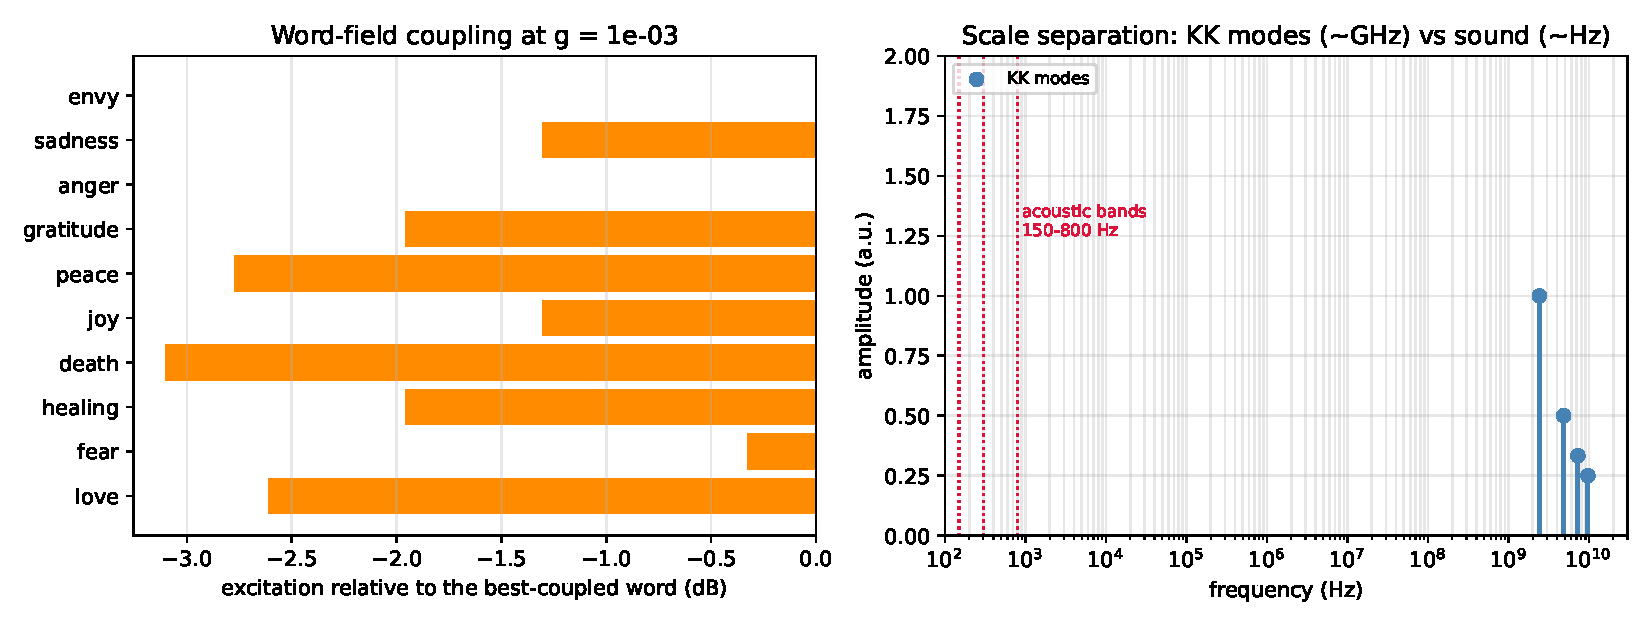
\includegraphics[width=0.9\textwidth]{figures/fig06_word_excitation.pdf}
\caption{Links: die relative Wort-Feld-Kopplung für die zehn in der Arbeit verwendeten Bänder. Rechts: die Skalentrennung zwischen den KK-Moden (~GHz) und den akustischen Bändern (~Hz).}
\label{fig:cuvant}
\end{figure}

\subsection{Zeit als Schwingung}
Die Definition der Sekunde: „Eine Sekunde ist die Dauer von 9.192.631.770 Perioden der Strahlung des Caesium-133-Atoms.`` Was geschieht, wenn sich die Frequenz ändert: Steigt die Frequenz, wird die Zeit gestaucht; sinkt sie, wird die Zeit gedehnt. Die Schumann-Resonanz: historisch $\sim 7,83$ Hz, in jüngerer Zeit $\sim 12$ Hz. Das Herz als biologische Uhr: Angst ($\sim 120$ bpm) --- die Zeit fliegt; Meditation ($\sim 50$ bpm) --- die Zeit ist gedehnt; Tiefschlaf ($\sim 40$ bpm) --- die Zeit verschwindet. Relative, nicht absolute Bezüge: Caesium (9.192.631.770 Hz), Schumann (7,83--12 Hz), das Herz (1,2 Hz). Sie alle sind relativ. Keiner von ihnen ist „der wahre``.
\begin{equation}
\text{Reality} = \frac{\text{Change}}{\text{Reference}}
\end{equation}

\subsection{Multiple Realitäten und das Multiversum}
Das gesamte Akasha-Feld: $A_{\text{total}} = \sum_{k=1}^{N_{\text{vacua}}} A_k$. Der Zustand des Multiversums: $|\Psi_{\text{multiverse}}\rangle = \otimes_{k=1}^{N_{\text{vacua}}} |A_k\rangle$. Die Schnittmenge der Realitäten: Realitäten sind nicht nur parallel --- sie können sich schneiden.

\subsection{Die universelle Bibliothek (Akasha)}
Der Inhalt des Feldes: Das Akasha-Feld enthält alle Information --- alles, was war, alles, was ist, alles, was sein wird.
\begin{equation}
A_{\text{total}} = \sum_{\text{(all events)}} A_i
\end{equation}
Der Zugang zur Information:
\begin{equation}
I_{\text{access}}(t) = \int_0^\infty S_A(\omega) S_G(\omega, t) d\omega
\end{equation}
Die Indexierung: Information wird nach Relevanz indexiert, nicht nach Zeit.
\begin{equation}
\text{Information received} = \text{Akashic field} \times \text{Relevance}(t)
\end{equation}

\subsection{Die Hierarchie des Empfangs}
\begin{table}[H]
\centering
\begin{tabular}{@{}clcc@{}}
\toprule
\textbf{Ebene} & \textbf{System} & \textbf{$\Phi$} & \textbf{Zugang} \\ \midrule
0 & Thermostat & 0 & Keiner \\
1 & C. elegans & Minimal & Chemotaxis \\
2 & Insekt & Niedrig & Empfindung \\
3 & Maus & Mäßig & Emotion \\
4 & Hund & Hoch & Empathie \\
5 & Corvide & Hoch & Planung \\
6 & Oktopode & Verteilt & Problemlösen \\
7 & Mensch & Sehr hoch & Selbstbezug \\
8 & Trainierter Mensch & Erweitert & Metakognition \\ \bottomrule
\end{tabular}
\end{table}
Die Grenze des Empfangs: $\lim_{\Phi \rightarrow \infty} E(\Phi) = I_{\text{total}}$.

\subsection{Das Wort als Ursprung: die Konvergenz der Religionen}
Alle großen religiösen Traditionen beschreiben das Wort als Ursprung des Universums. Das Christentum kennt den Logos --- das Wort (die fundamentale Mode des Feldes). Der Hinduismus kennt Om (die Urschwingung). Der Islam kennt Kun („Sei!``).

\subsection{Die akustische Manifestation des Akasha-Feldes}
$A(x,t) = \sum_n A_n \cos(\omega_n t + \varphi_n)$. Das akustische Spektrum: $\omega_n = \frac{1}{R} \sqrt{n^2 + \mu_A^2 R^2}$.

\subsection{Gott in ART-12D}
Es gibt vier Hypothesen. Gott ist das Akasha-Feld selbst. Gott ist die Quelle des Feldes. Gott ist das universelle Bewusstsein. Gott ist eine menschliche Projektion. Ich weiß nicht, welche richtig ist. Aber die Frage ist legitim.

\subsection{Dunkle Materie und Dunkle Energie: zwei Gesichter desselben Feldes}
Die ART-12D-Hypothese: Dunkle Materie und Dunkle Energie sind zwei Aspekte desselben Akasha-Feldes. Formalisierung:
\begin{equation}
L_A = \frac{1}{2} g^{MN} \partial_M A^* \partial_N A + \frac{1}{2} \mu_A^2 |A|^2 - \frac{\lambda_A}{4} |A|^4
\end{equation}
Die Zustandsgleichung: $w = p_A / \rho_A$. Für ein oszillierendes Feld wird das Zeitmittel exakt entlang der Bahn berechnet und hängt vom Verhältnis $\delta = A_{\text{osc}}/A_{\min}$ zwischen Schwingungsamplitude und dem Wert des Potentials im Minimum ab. Es gibt drei verschiedene Regime:
\begin{center}
\begin{tabular}{@{}lll@{}}
\toprule
\textbf{Regime} & \textbf{Bedingung} & $w$ \\ \midrule
Kleine Schwingung um das Minimum & $\delta \ll 1$ & $0$ (Materie) \\
Schwingung, vom quartischen Term dominiert & $\delta \gg 1$ & $1/3$ (Strahlung) \\
Erstarrtes Feld im Minimum & $\delta = 0$ & $-1$ (kosmologische Konstante) \\ \bottomrule
\end{tabular}
\end{center}
Version 30 behauptete, das Regime großer Amplitude ergebe $w \simeq 1$. Der korrekte Wert ist $1/3$: Das Virialtheorem liefert $\langle K \rangle = 2\langle V \rangle$ für ein quartisch dominiertes Potential. Der Wert $w = 1$ entspricht der kinetischen Dominanz (Kination), die von den quartischen Schwingungen nicht erreicht wird, während $w = -1$ dem erstarrten Feld entspricht, nicht kleiner Amplitude.
